\lesson{3}{Oct 6 2021 Wen (08:43:42)}{Quantization of Energy}{Unit 2}

When elements are heated or energized, their electrons absorb energy and transition to a higher energy level. This is their excited state. Eventually, electrons fall back to a lower orbit or their ground state; but when they do, they release energy in the form of light. This light appears in different colors, depending on the frequency and wavelength of the light released.

When this light is analyzed using a spectroscope, a unique set of colored lines called an emission spectrum identifies the element. This is the emission spectrum for the element hydrogen.

Bohr's model of the hydrogen atom showed the electrons traveling in specific orbits, or paths, around the nucleus.

He suggested that the electrons have a fixed amount of potential energy related to each orbit. The closer the orbit is to the central nucleus, the lower the electron's potential energy.

When you climb a ladder, your potential energy changes depending on your position in relation to the ground.

The higher you climb, the farther you can fall.

This can be compared to the orbits of Bohr's model. Each orbit has its own small, definite amount of potential energy; scientists say that this energy is quantized.

Just like the high rungs of a ladder, the higher orbits of an atom are not as stable for an electron.

The electrons eventually fall back to a lower orbit, closer to the nucleus.

\subsubsection*{Determining the energy of photons}

Planck's hypothesis about energy and quanta led to the discovery of the photon. A photon is a basic particle representing a quantum of energy, E. A photon of light is emitted by an atom when an electron within the atom transitions to a lower energy level. Conversely, a photon of energy is absorbed by an atom when an electron within the atom moves to a higher energy level. Because energy is transferred in quanta, the photon's entire energy is transferred, not just a fraction of it.
    
\begin{marginfigure}
    \centering
    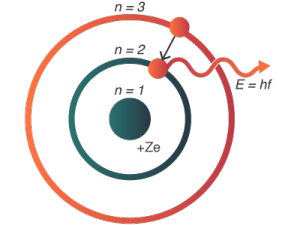
\includegraphics[width=\textwidth,height=\textheight,keepaspectratio]{images/energy-of-photons}
    \sidecaption{Here is what the energy of the photon looks like.}
    \label{fig:energy-of-photons}
\end{marginfigure}

\begin{definition}[Planks Constant]
    \begin{align}
        E = hf
    \end{align}

    The energy of a photon is directly proportional to the frequency of the photon's emission or absorption. Energy is measured in Joules, $h$ is Planck's constant of $6.626 \times 10^{-34} \times s$, and $f$ is the frequency of the energy.
\end{definition}

The amount of energy in a photon is influenced by the frequency of its energy source. Examine the electromagnetic spectrum chart below. Notice that as the frequency of energy decreases, the energy of photons from that source also decreases. Because of the inverse relationship between frequency and wavelength, when the wavelength of energy decreases, the energy of photons from that source increases.

\newpage
